\section{空间点、直线、平面之间的位置关系}

本节要点:
\begin{itemize}
    \item 掌握确定平面的4种方法。
    \item 掌握直线与平面之间的位置关系。
\end{itemize}

~

三维空间的基本元素可以分为点、线、面,高中阶段讨论的是直线和平面。

8.4.1主要讲了如何确定一个平面:
\begin{itemize}
    \item 三点;
    \item 直线+一点;
    \item 两条相交线;
    \item 两条平行线。
\end{itemize}
这些是解题时,构建平面的方法。

8.4.2主要讲了直线与平面之间的位置关系:
\begin{itemize}
    \item 直线与直线的关系:相交,平行,异面;
    \item 直线与平面的关系:属于,相交,平行;
    \item 平面与平面的关系:相交,平行。
\end{itemize}
教材对线面关系没有明确的定义、定理和性质,但类似的概念点较多,相互间逻辑关系非常复杂。万变不离其宗,还是要从最基本的点面关系出发,体会并深刻理解点面关系,多画图。

~

\begin{example}[综合运用8,难度:$\star $]
如图,$\bigtriangleup ABC$在平面$\alpha $外,$AB\cap \alpha =P,BC\cap \alpha =Q,AC\cap \alpha =R$,求证:$P,Q,R$三点共线。
\end{example}

\begin{figure}[h]
\centering
\begin{tikzpicture}[style={x={(-135:0.5)},y={(1cm,0)},z={(0,1cm)}}, line join=round, scale=0.5]
\draw (3,-4,0)--(3,4,0)--(-3,4,0)--(-3,-4,0)--(3,-4,0);
\coordinate[label=below:{$R$}] (R) at (0,0,0);
\coordinate[label=below:{$Q$}] (Q) at (1,-2,0);
\coordinate[label=below:{$P$}] (P) at (-1,2,0);
\coordinate[label=above:{$A$}] (A) at (0,0,3);
\coordinate[label=right:{$B$}] (B) at ($(A)!0.33!(P)$);
\draw[thick] (A)--(P);
\draw[thick,name path=l1] (A)--(R);
\draw[thick,name path=l2] (Q)--(B);
\path [name intersections={of=l1 and l2}] coordinate[label=above left:$C$] (C) at (intersection-1);
\draw[thick,dashed,blue] (Q)--(P);
\end{tikzpicture}
\end{figure}


解:

即找到一个平面,$P,Q,R$三点在该平面上,且该平面和$\alpha $相交。令$\bigtriangleup ABC$所在的平面为$\beta $,则易得$\alpha $和$\beta $相交,令交线为$l$。
\begin{align*}
&\because P\subset AB\Rightarrow P\subset \beta \\
&\because P\subset \alpha \\
&\therefore P\subset \alpha \cap \beta =l
\end{align*}
同理可得$Q,R\subset l$,证毕。

\begin{tcolorbox}
本题看似考察点面关系,实则考察面面关系。
\end{tcolorbox}

~

\begin{example}[拓广探索9,难度:$\star $]
如图是一个正方体的展开图,如果将它还原为正方体,那么在$AB,CD,EF,GH$这四条线段中,哪些线段所在的直线是异面直线?
\end{example}

\begin{figure}[h]
\centering
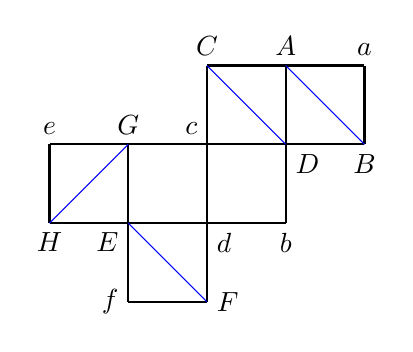
\begin{tikzpicture}[line join=round, scale=1]
\coordinate[label=above:      {$e$}] (e) at (-2,0);
\coordinate[label=above:      {$G$}] (G) at (-1,0);
\coordinate[label=above left: {$c$}] (c) at (0,0);
\coordinate[label=below right:{$D$}] (D) at (1,0);
\coordinate[label=below:      {$B$}] (B) at (2,0);
\coordinate[label=above:      {$C$}] (C) at (0,1);
\coordinate[label=above:      {$A$}] (A) at (1,1);
\coordinate[label=above:      {$a$}] (a) at (2,1);
\coordinate[label=below:      {$H$}] (H) at (-2,-1);
\coordinate[label=below left: {$E$}] (E) at (-1,-1);
\coordinate[label=below right:{$d$}] (d) at (0,-1);
\coordinate[label=below:      {$b$}] (b) at (1,-1);
\coordinate[label=left:       {$f$}] (f) at (-1,-2);
\coordinate[label=right:      {$F$}] (F) at (0,-2);
\draw[thick] (C)--(a) (e)--(B) (H)--(b) (f)--(F);
\draw[thick] (e)--(H) (G)--(f) (C)--(F) (A)--(b) (a)--(B);
\draw[blue] (G)--(H) (E)--(F) (C)--(D) (A)--(B);
\end{tikzpicture}
\end{figure}

解:

需要将展开图还原,标记剩余顶点方便还原,以$dcbD$平面为底,结果如下,余下略。

\begin{figure}[h]
\centering
\begin{tikzpicture}[style={x={(-145:0.5)},y={(1cm,0)},z={(0,1cm)}}, line join=round, scale=2]
\mydrawcube[1]{d}{B}{D}{c}{E}{H}{A}{C}
\draw[blue] (E)--(B)--(A) (H)--(C)--(D);
\coordinate[label=below:{$F$}] (F) at (B);
\coordinate[label=above:{$G$}] (G) at (C);
\end{tikzpicture}
\end{figure}

\begin{tcolorbox}
本题需要空间想象力,较难。还原时,尽量减少翻折次数,以降低难度,所以选$dcbD$平面为底。
\end{tcolorbox}




